% THIS IS SIGPROC-SP.TEX - VERSION 3.1
% WORKS WITH V3.2SP OF ACM_PROC_ARTICLE-SP.CLS
% APRIL 2009
%
% It is an example file showing how to use the 'acm_proc_article-sp.cls' V3.2SP
% LaTeX2e document class file for Conference Proceedings submissions.
% ----------------------------------------------------------------------------------------------------------------
% This .tex file (and associated .cls V3.2SP) *DOES NOT* produce:
%       1) The Permission Statement
%       2) The Conference (location) Info information
%       3) The Copyright Line with ACM data
%       4) Page numbering
% ---------------------------------------------------------------------------------------------------------------
% It is an example which *does* use the .bib file (from which the .bbl file
% is produced).
% REMEMBER HOWEVER: After having produced the .bbl file,
% and prior to final submission,
% you need to 'insert'  your .bbl file into your source .tex file so as to provide
% ONE 'self-contained' source file.
%
% Questions regarding SIGS should be sent to
% Adrienne Griscti ---> griscti@acm.org
%
% Questions/suggestions regarding the guidelines, .tex and .cls files, etc. to
% Gerald Murray ---> murray@hq.acm.org
%
% For tracking purposes - this is V3.1SP - APRIL 2009

\documentclass{acm_proc_article-sp}

\begin{document}

% set the path for graphics
\graphicspath{{figures/}}

\title{User-Device Physical Unclonable Functions (UD-PUFs) based on Mobile Device Touchscreen Pressure}
%\subtitle{[Extended Abstract]
%\titlenote{A full version of this paper is available as
%\textit{Author's Guide to Preparing ACM SIG Proceedings Using
%\LaTeX$2_\epsilon$\ and BibTeX} at
%\texttt{www.acm.org/eaddress.htm}}}
%
% You need the command \numberofauthors to handle the 'placement
% and alignment' of the authors beneath the title.
%
% For aesthetic reasons, we recommend 'three authors at a time'
% i.e. three 'name/affiliation blocks' be placed beneath the title.
%
% NOTE: You are NOT restricted in how many 'rows' of
% "name/affiliations" may appear. We just ask that you restrict
% the number of 'columns' to three.
%
% Because of the available 'opening page real-estate'
% we ask you to refrain from putting more than six authors
% (two rows with three columns) beneath the article title.
% More than six makes the first-page appear very cluttered indeed.
%
% Use the \alignauthor commands to handle the names
% and affiliations for an 'aesthetic maximum' of six authors.
% Add names, affiliations, addresses for
% the seventh etc. author(s) as the argument for the
% \additionalauthors command.
% These 'additional authors' will be output/set for you
% without further effort on your part as the last section in
% the body of your article BEFORE References or any Appendices.

\numberofauthors{3} %  in this sample file, there are a *total*
% of EIGHT authors. SIX appear on the 'first-page' (for formatting
% reasons) and the remaining two appear in the \additionalauthors section.
%
\author{
% 1st. author
\alignauthor Timothy M. Dee\\
       \affaddr{Electrical \& Computer Engineering}\\
       \affaddr{Iowa State University}\\
       \affaddr{Ames, IA, USA}\\
       \email{deetimothy33@gmail.com}
% 2nd. author
%\alignauthor Ian T. Richardson\\
%       \affaddr{Electrical \& Computer Engineering}\\
%       \affaddr{Iowa State University}\\
%       \affaddr{Ames, IA, USA}\\
%       \email{ian.t.rich@gmail.com}
% 3nd. author
\alignauthor Akhilesh Tyagi\\
      \affaddr{Electrical \& Computer Engineering}\\
      \affaddr{Iowa State University}\\
       \affaddr{Ames, IA, USA}\\
       \email{tyagi@iastate.edu}
}

%\date{30 July 1999}
% Just remember to make sure that the TOTAL number of authors
% is the number that will appear on the first page PLUS the
% number that will appear in the \additionalauthors section.

\maketitle
\begin{abstract}
%TODO remove the last sentence, mabe? Also, include numbers describing important results
Described in this document is a physical unclonable function (PUF) utilizing the variability derived from the pressure with which users interact with their mobile device touchscreens. We illustrate how a sequence of these pressure values from discrete touchscreen interactions may be used to uniquely characterize a user-device pair. This characterization method may find many applications in protecting access to a mobile device from a malicious party. As a result, the effectiveness of this scheme is described in terms of how one user may be differentiated from another.
\end{abstract}

% A category with the (minimum) three required fields
%\category{H.4}{Information Systems Applications}{Miscellaneous}
%A category including the fourth, optional field follows...
%\category{D.2.8}{Software Engineering}{Metrics}[complexity measures, performance measures]

%\terms{Theory}

%\keywords{physical unclonable function (PUF), user device physical unclonable function (UD-PUF)} % NOT required for Proceedings

\section{Introduction}
\label{sec:intro}
%Motivate the reasoning behind why we may want to secure mobile devices more
Mobile devices are ubiquitous in the modern world. These devices are becoming progressively more important for many applications with security sensitive data. 
Securing mobile devices poses unique challenges and opportunities compared to traditional data security where it is difficult for an attacker to access the physical device on which the data is stored or from which the sensitive data may be accessed. Although there is increased probability that a device may be compromised, there is also greater number of available sensors to measure the variability in the way users interact with mobile devices compared compared to conventional computing technology.
%

%develop an understanding of the need for this system
The reality that an attacker may be able to gain access to a physical device makes securing any data stored on or accessed by a mobile device significantly more challenging. Traditional physical unclonable functions (PUFs) which can only be used to uniquely to a given hardware device are no longer sufficient to guarantee the authenticity of a user.
%
This motivates an extension of the traditional PUF known as a user-device physical unclonable function(UD-PUF). This UD-PUF entangles the physical characteristics of the user in combination with the device to enable a more secure authentication scheme.

%problem statement, describe what the UD-PUF must accomplish 
A UD-PUF is a function of both the hardware of a given device and the user of that device. Such a function must change significantly given unique user-device pairs, thus we must identify a property or properties which vary among mobile device hardware and a property or properties which vary among users of a given device. The best candidates to use will be properties which present with the most variability, and properties which are most easily exposed to the android operating system.

%problem statement continued, what must be the properties of the authentication system.
Identifying properties of device and user which can be used to construct our UD-PUF is insufficient; the system must also be practical under normal use conditions for mobile devices. The system must be non-intrusive to the user, fast enough to run on mobile devices, and accurate when authenticating users. If a user must spend a long time authenticating they are not able to use this time to accomplish the task for which they are being authenticated, this detracts from the efficiency of using a mobile device to complete the task. If the proposed system is too computationally intense to be run on a mobile device, or the system is only accurate some low percentage of the time then it is useless for any practical application. For these reasons we propose a system which operates under a continuous authentication scheme.

%describe in depth the continuous authentication scheme proposed, this is where the main contributions of this work should be discussed
While other solutions have shown that a user may be distinguished by using data from several different sensors, this paper establishes that variability in the way in which users interact with the touch screen may be enough to differentiate one user from another. In other words there is a single source of information which is also tied to the usability of the device. A failue of the touchscreen to function also constitues a failure in the device as a whole. Thus the system is robust because it will only fail upon failure of the device. Compare this to other systems whose functionality depends on many components. A failure in one of these components disrupts the authentication scheme making these systems more prone to failure. 

% describe the structure of the paper, what is contained in each section
The structure of the paper is as follows. Section \ref{sec:related_work} discusses some related work. Touchscreen pressure and what it measures are described in section \ref{sec:touchscreen}. Reasons for choosing a given modeling scheme for users and devices is discussed in section \ref{sec:modeling}. Section \ref{touch_pressure_modeling} provides some implementation details with respect to how touchscreen pressure is used in the modeling scheme. Data collection methods are discussed in section \ref{sec:data_collection}. The authentication scheme is discussed in section \ref{sec:differentiation}. The results including final numbers and suggestions in practical applications are articulated in section \ref{sec:results}. Conclusions are presented in section \ref{sec:conclusions}. Finally section \ref{sec:futurework} discusses future work in this area. 

\section{Related Work}
\label{sec:related_work}
%detail what was done in the sensec paper
SenSec, a similar authentication scheme to the one proposed in this paper, completed at Carnegie Mellon used information from from accelerometers, gyroscopes and magnetometers to construct a model of a user. \cite{zhu2013sensec} This method can be classified as a UD-PUF as each accelerometer, gyroscope and magnetometer will have some variance inherent in the manufacturing process for these devices \cite{?}; the input to these devices will also vary significantly by user \cite{?}. As a result the output is a function which varies with changes in user or device, a UD-PUF.

%TODO more about sensec, relate things in sensec back to our work
%TODO explain what we can learn from sensec use of marcov chain
Another noteable aspect of the SenSec system is their method of modeling users with an n-order Markov Chain. This system presents several benefits which, according to sensec include, relative simplicity and scaleability. \cite{zhu2013sensec} 

\cite{shi2011senguard}
\cite{feng2012continuous}

%provide a brief history of UD-PUFS
%explain why are solution is better than previous/other solutions

%describe what touchscreen pressure is
%describe the physical component of the pressure (current at the edge of screen on android device)
\section{Touchscreen Pressure}
\label{sec:touchscreen}
%describe what is touchscreen pressure
If our goal is be be able to distinguish a user's interaction with a given device from this same user on a different device and from different users on any device than our description of the user will need to be a product of both the user and the device. In the android operating system there exists a pressure function which returns a value proportional to current at sides of phone for a given touch screen interaction. \cite{zhu2013sensec} This is the value which will serve as the basis for our scheme and will henseforth be referred to as touch pressure. 

%describe why touchscreen pressure is a good candidate for our UD-PUF
The pressure function is significant because it's value not only depends on the characteristics of the device but also on the way in which a user interacts with a given device. The effect of a given device on the touch pressure value will differ significantly due to variations implicit in the manufacturing process for the touchscreens of these devices. \cite{manufacturing_differences} Our supposition is a given user will interact with a touchscreen in such a way as to cause significant variations in the touch pressure values when compared to other users on the same touchscreen \cite{user_touchscreen_interations}.  Given this, we have chosen touch pressure as the basis for our UD-PUF.

%describe a marcov model in general
%describe what it means to be an n-gram sliding marcov model
%describe in what way we a marcov model to describe a user, device pair (our marcov model of touch, pressure values.
%An n-gram sliding marcov model.
\section{Modeling a User-Device Pair}
\label{sec:modeling}
%describe the motivation for the use of a marcov chain
Interactions between users and devices are complex. To interpret these actions in a meaningful way, in order to perform an authentication for example, it is necessary to simplify these interactions. The chosen model must provide sufficient entropy such that a model generated with a given user-device pair is not consistently reproducible by another user or on a different device. The modeling method must also be easily reproducible by the original user on the original device. A model having the necessary characteristics required for this application is a Markov Chain.

%TODO describe what is a marcov chain
Markov Chains are useful in predicting systems whose behavior can be modeled in discrete states. The transitions between states can be identified to happen with some probability.

%Other information about marcov chains
%TODO traditional use of marcov chains
Historically the Marcov Chain has found applications in (statistics?)

Upon identification of an appropriate model the next step is to discover an optimal way in which it may be applied to the current problem. An interaction between a user and device can be described as a sequence of touch pressure values. Using a Markov Chain to describe this sequence is only reasonable if we suppose that a given touch pressure value depends on some number of preceding touch pressure values. \cite{marcov_chains_previous_n_values}
%

%n-gram a continuious sequence of n items
%markov model for comparason is built from a sliding model of the previous n touches
%describe how the marcov chain is applied to touch pressure to model a user
%this is a description of our specific implementation of a marcov model
\section{Touch Pressure Modeling}
\label{touch_pressure_modeling}
%TODO this section should describe various implementation details
%
%describe the marcov model used
The goal in modeling a system with a markov model is to classify the system in terms of its transitions between states. If such a model is to be used to purposes of uniquely identifying a given system, than the states of the model must be chosen in a way which exposes the uniqueness of the system.
The states of our markov model are defined by the range in which

%TODO TODO describe aspects of the implementation

\section{Data Collection}
\label{sec:data_collection}
%TODO
%describe the number of users from which the data was collected
%describe the method of collection
Data for creating touch pressure models in this experiment was generated using a special keyboard application for the android operating system. Users would load the keyboard onto their device and continue using the device in the way they would normally. Some users were asked to play a typing game in order to help expedite the data collection process. After the users had generated at least ten thousand touches the data was collected from the user's device.
%put the data in context by detailing the number of touches collected from each user and the number of touches used to build the model

%basically the authentication scheme used
%frame it in more general terms, independent of our specific application
\section{Differentiating User-Device Pairs}
\label{sec:differentiation}

%this figure describes how false positive and false negative percentages vary based on authentication threshold
\begin{figure}
\centering
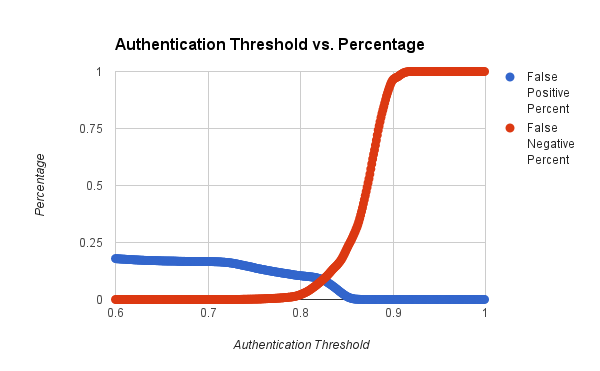
\includegraphics[width=3.9in]{threshold_vs_percentages.png}
\caption{Describes how false positive and false negative percentages vary as the authentication threshold is adjusted.}
\label{fig:threshold_vs_percentages}
\end{figure}

%TODO
%describe what the authentication threshold is
%define false positive
%define false negative
%explain why the intersection of these two is significant in choosing the authentication threshold
In distinguishing a particular user from another different user, it is necessary to develop a method of comparison between users. In our method of comparison we take the probability associated with a touch pressure coming after a sequence of preceding touch pressures for a particular user and compute the difference between this probability and the probability of the same touch pressure coming after the same sequence of touches for a different user. The average of these probability differences is taken to be the difference between two users.
%
Once a comparison is established a natural extension is a system of authentication. This system needs to determine when two sets of touch pressure values came from the same user-device pair. When authenticating a user, we take one minus the average difference between the model constructed from the two sets of touch pressure values. Take this value to be the authentication percentage for a given set of touch pressure values against another.
%
%TODO TODO add more metrics, and explain them, provide more graphs about them
To determine how well this system does at differentiating users it is useful to develop metrics which describe the system's performance under conditions which are similar to it's potential real-world applications. Figure \ref{fig:threshold_vs_percentages} illustrates how false positive percentage and false negative percentage vary based on where the threshold for authentication is set. 

%authentication threshold described
Here, authentication threshold refers to the value of authentication percentage one model must have against another for the models to be considered the same; two models which are the same are supposed to have been created from touches generated by the same user-device pair.
%false positive percentage described
False positive percentage measures what fraction of authentications between two sets of touch pressures which did not come from the same user-device pair, therefore these sets should not be considered the same, but did authenticate as being the same in our authentication system.
%false negative percentage described
False negative percentage is exactly the inverse of false positive percentage in that it describes what fraction of authentications between two sets of touch pressures which did come from the same user-device pair, but did not authenticate as being the same in our authentication system.

%significance of the intersection of false positive, false negative values
In Figure \ref{fig:threshold_vs_percentages} there exists a clear intersection between false negative and false positive percentages. This intersection is significant; at this point the system neither biased toward allowing user-device pairs which should not authenticate to pass authentication nor toward disallowing user-device pairs, which should authenticate, from passing authentication. This point represents a balance in design, but the best authentication threshold will depend on the application of this system.

%what number of states exposed the most uniqueness e.g. how many tokens were best
%with what accuracy could users be distinguished from one-another
\section{Results}
\label{sec:results}

%this section describes how authentication accuracy was investigated. Also included are a few figures which describe the best authentication accuracy percentage
\begin{figure}
\centering
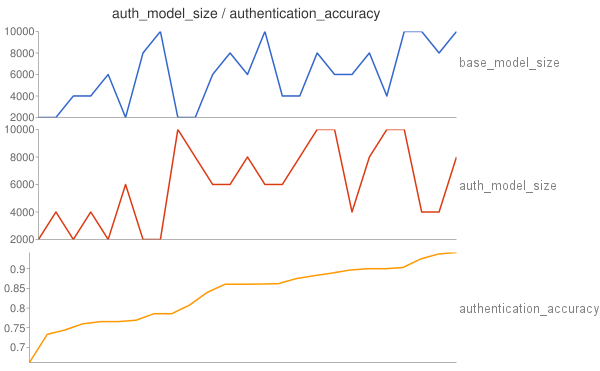
\includegraphics[width=3.9in]{authentication_accuracy_vs_model_size.png}
\caption{Authentication accuracy is a function of both the base model size and authentication model size.}
\label{fig:authentication_accuracy}
\end{figure}

%explain the contents of this figure.
%explain what each of the metrics used in the figure are.
%
In exploring the design space of this system we are trying to determine how well the system will perform in the end use case. Perhaps the best measure of the system's performance is how accurate the system is when authenticating users. Figure \ref{fig:authentication_accuracy} depicts authentication\_accuracy as a function of base\_model\_size, number of touches known to have originated from an authentic user, and auth\_model\_size, number of touches which are to be checked against the model generated from the base touches. We define authentication\_accuracy to be the percentage of authentications for which our system makes the correct decision. In other words, an authentic user is authenticated and a non-authentic user is not authenticated. The size of base model and user model which result in a given authentication accuracy are aligned with that authentication accuracy on the horizontal axis in the chart. 

\begin{figure}
\centering
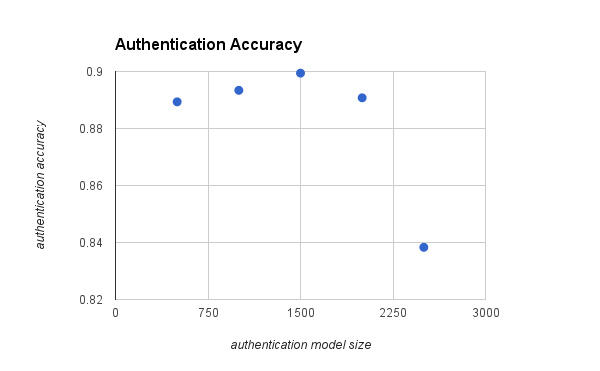
\includegraphics[width=3.9in]{extensive_authentication_accuracy.png}
\caption{Depicts the result of many model comparisons done around the area of best results in Figure \ref{fig:authentication_accuracy}.}
\label{fig:extensive_authentication_accuracy}
\end{figure}

%explain the contents of this figure.
%explain what each of the metrics used in the figure are.
%
To establish that the results in Figure \ref{fig:authentication_accuracy} hold for large numbers of comparisons many more comparisons where done around the area of best results. The results of these tests are presented in Figure \ref{fig:authentication:accuracy}. For the results depicted in the figure, user\_model\_size is held constant at ten thousand while auth\_model\_size is varied. The test was performed in this way because variations in auth\_model\_size seems to have a greater impact on authentication accuracy than variations in base\_model\_size. Approximately the same trend as seen in Figure \ref{fig:authentication_accuracy} presents itself in Figure \ref{fig:extensive_authentication_accuracy}.

\section{Conclusions}
\label{sec:conclusions}
%describe what has been presented in the paper
This paper presents an approach toward continuous authentication which utilizes the variability in the way users interact with the touchscreens of their devices to differentiate distinct user-device combinations. We model these interactions with an n-gram Markov model which allows us to describe the likelihood that two sequences of touch pressure values came from the same user in a probabilistic fashion. Data for this approach comes from the user's interactions with the touchscreen of their device. This data will be generated over time by the user; thus this scheme lends itself very well to a continuous authentication model.

%TODO describe the design space for the system presented in the paper
Depending on the implementation of this system, varying the parameters of the modeling system can allow the implementer to tune the system to their specific purpose. 

%possible, describe applications  in terms of continuous authentication
\section{Future Work}
\label{sec:futurework}

\bibliographystyle{abbrv}
\bibliography{bibliography/marcov_chains,bibliography/pufs,bibliography/other}
\end{document}
